%%%%%%%%%%%%%%%%%%%%%%%%%%%%%%%%%%%%%%%%%
% Beamer Presentation
% LaTeX Template
% Version 1.0 (10/11/12)
%
% This template has been downloaded from:
% http://www.LaTeXTemplates.com
%
% License:
% CC BY-NC-SA 3.0 (http://creativecommons.org/licenses/by-nc-sa/3.0/)
%
%%%%%%%%%%%%%%%%%%%%%%%%%%%%%%%%%%%%%%%%%

%----------------------------------------------------------------------------------------
%	PACKAGES AND THEMES
%----------------------------------------------------------------------------------------

\documentclass{beamer}

\mode<presentation> {

% The Beamer class comes with a number of default slide themes
% which change the colors and layouts of slides. Below this is a list
% of all the themes, uncomment each in turn to see what they look like.

%\usetheme{default}
%\usetheme{AnnArbor}
%\usetheme{Antibes}
%\usetheme{Bergen}
%\usetheme{Berkeley}
%\usetheme{Berlin}
%\usetheme{Boadilla}
\usetheme{CambridgeUS}
%\usetheme{Copenhagen}
%\usetheme{Darmstadt}
%\usetheme{Dresden}
%\usetheme{Frankfurt}
%\usetheme{Goettingen}
%\usetheme{Hannover}
%\usetheme{Ilmenau}
%\usetheme{JuanLesPins}
%\usetheme{Luebeck}
%\usetheme{Madrid}
%\usetheme{Malmoe}
%\usetheme{Marburg}
%\usetheme{Montpellier}
%\usetheme{PaloAlto}
%\usetheme{Pittsburgh}
%\usetheme{Rochester}
%\usetheme{Singapore}
%\usetheme{Szeged}
%\usetheme{Warsaw}

% As well as themes, the Beamer class has a number of color themes
% for any slide theme. Uncomment each of these in turn to see how it
% changes the colors of your current slide theme.

%\usecolortheme{albatross}
%\usecolortheme{beaver}
%\usecolortheme{beetle}
%\usecolortheme{crane}
%\usecolortheme{dolphin}
%\usecolortheme{dove}
%\usecolortheme{fly}
%\usecolortheme{lily}
%\usecolortheme{orchid}
%\usecolortheme{rose}
\usecolortheme{seagull}
%\usecolortheme{seahorse}
%\usecolortheme{whale}
%\usecolortheme{wolverine}

%\setbeamertemplate{footline} % To remove the footer line in all slides uncomment this line
%\setbeamertemplate{footline}[page number] % To replace the footer line in all slides with a simple slide count uncomment this line

%\setbeamertemplate{navigation symbols}{} % To remove the navigation symbols from the bottom of all slides uncomment this line
}



\newcommand\Fontvi{\fontsize{6}{7.2}\selectfont}
\newcommand\Fontvii{\fontsize{7}{8.2}\selectfont}
\newcommand\Fontviii{\fontsize{8}{9.2}\selectfont}

\usepackage{graphicx} % Allows including images
\usepackage{booktabs} % Allows the use of \toprule, \midrule and \bottomrule in tables

%----------------------------------------------------------------------------------------
%	TITLE PAGE
%----------------------------------------------------------------------------------------

\title[Drawdown project]{Monthly Presentation of Drawdown project} % The short title appears at the bottom of every slide, the full title is only on the title page

\author{Boying Gong, Xinyue Zhou} % Your name
\institute[UC Berkeley] % Your institution as it will appear on the bottom of every slide, may be shorthand to save space
{
University of California, Berkeley \\ % Your institution for the title page
\medskip
\textit{jorothy\_gong@berkeley.edu \\}
\textit{xinyue233@berkeley.edu} % Your email address
}
\date{\today} % Date, can be changed to a custom date

\begin{document}

\begin{frame}
\titlepage % Print the title page as the first slide
\end{frame}

\begin{frame}
\frametitle{Overview} % Table of contents slide, comment this block out to remove it
\tableofcontents % Throughout your presentation, if you choose to use \section{} and \subsection{} commands, these will automatically be printed on this slide as an overview of your presentation
\end{frame}

%----------------------------------------------------------------------------------------
%	PRESENTATION SLIDES
%----------------------------------------------------------------------------------------

%------------------------------------------------
\section{Description}
%------------------------------------------------

\begin{frame}
\frametitle{Asset Description}
\Fontviii
\begin{block}{US Equity}
\begin{itemize}
\item AGG: iShares Core US Aggregate Bond
\item HYG: iShares iBoxx \$ High Yield Corporate Bd
\item TIP: iShares TIPS Bond
\end{itemize}
\end{block}
\begin{block}{Index}
\begin{itemize}
\item BCOM: Bloomberg Commodity Index
\item G0O1: 3-Month U.S. Treasury Bill Index
\item MXEA: MSCI EAFE Index
\item MXEF: MSCI Emerging Markets Index
\item RAY: Russell 3000 Index
\item RMZ: MSCI US REIT Index
\item SPX: S\&P 500 Index
\item USGG10YR: US Generic Govt 10 Year
\end{itemize}
\end{block}
\end{frame}

%------------------------------------------------
\section{Summary of Assets}
%------------------------------------------------
\subsection{Returns}
%------------------------------------------------

\begin{frame}
\frametitle{Returns}
\Fontviii
\begin{columns}[c] % The "c" option specifies centered vertical alignment while the "t" option is used for top vertical alignment

\column{.35\textwidth} % Left column and width
\textbf{Heading}
\begin{enumerate}
\item Statement
\item Explanation
\item Example
\end{enumerate}

\column{.6\textwidth} % Right column and width
\begin{figure}[h]
\centering 
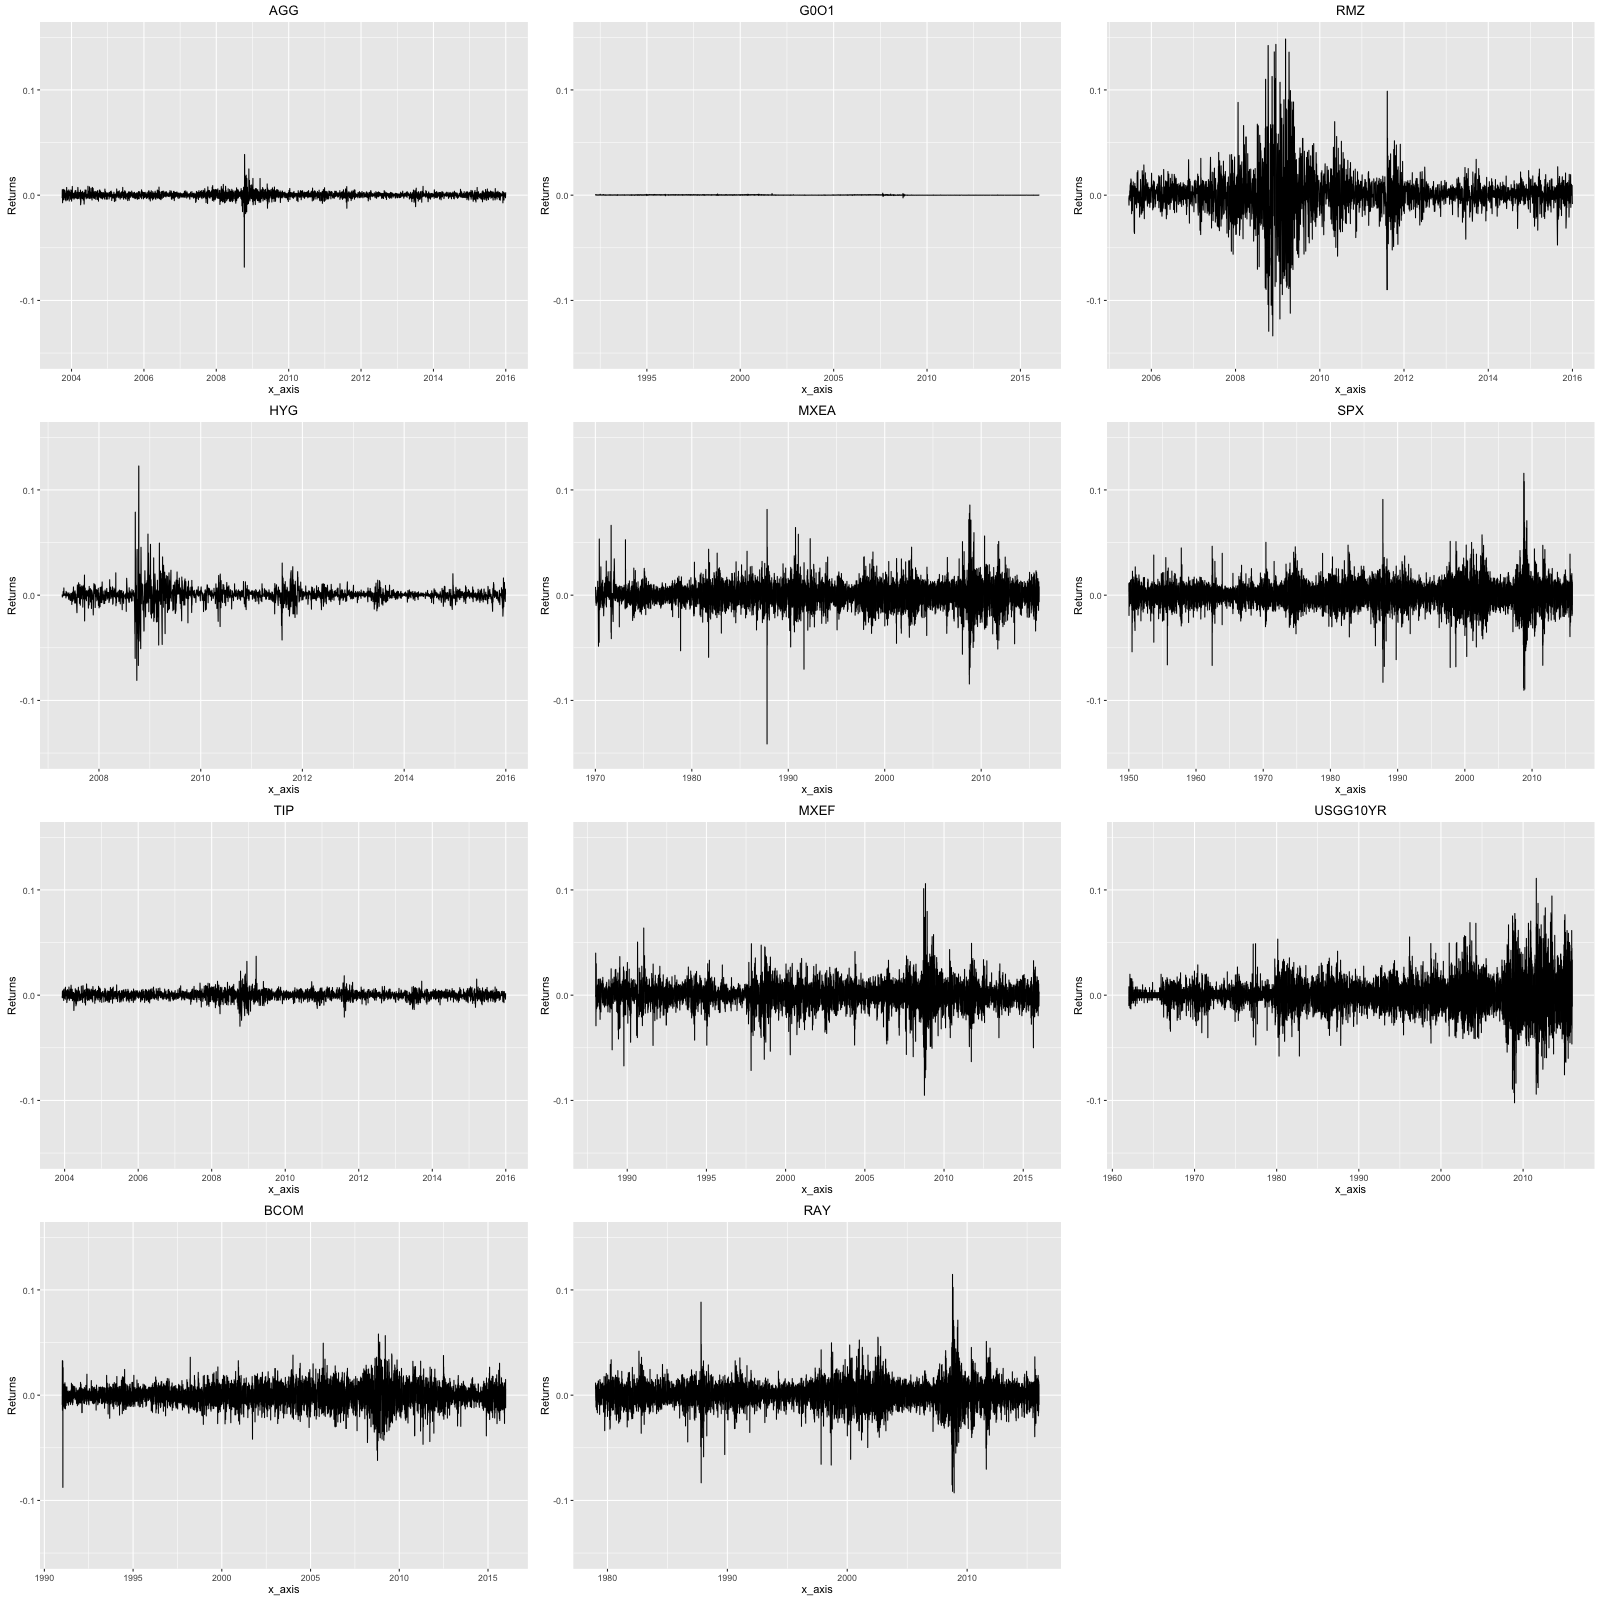
\includegraphics[width=6.5cm]{../results/returns}
\label{fig: dailyReturns}
\end{figure}
\end{columns}
\end{frame}

%------------------------------------------------

\begin{frame}
\frametitle{Return Distribution}
\Fontviii
\begin{columns}[c] % The "c" option specifies centered vertical alignment while the "t" option is used for top vertical alignment

\column{.35\textwidth} % Left column and width
\textbf{Heading}
\begin{enumerate}
\item Statement
\item Explanation
\item Example
\end{enumerate}

\column{.6\textwidth} % Right column and width
\begin{figure}[h]
\centering 
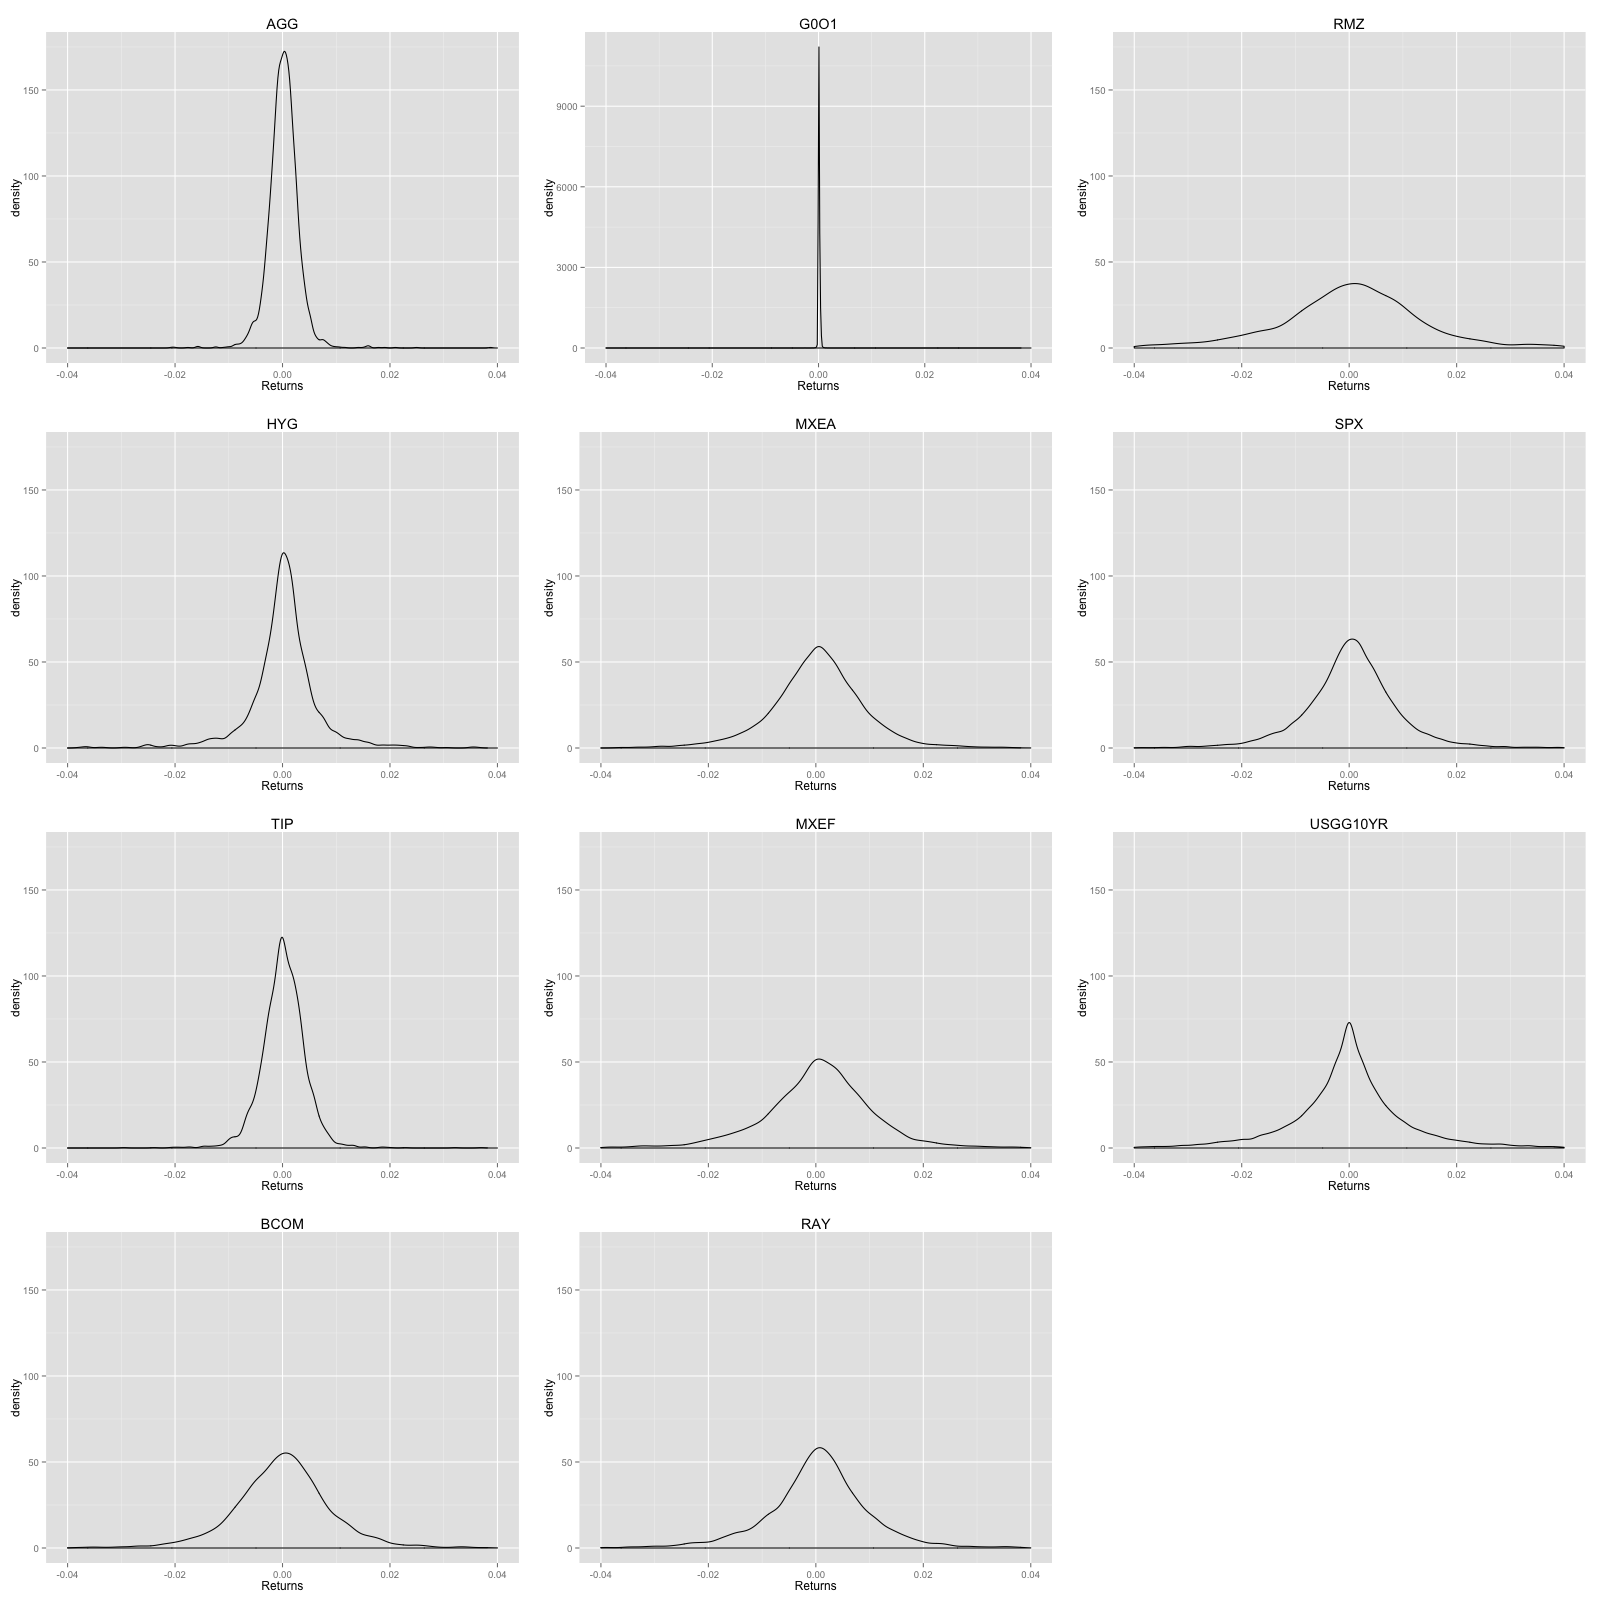
\includegraphics[width=6.55cm]{../results/returns_dist}
\label{fig: returnsDist}
\end{figure}
\end{columns}
\end{frame}


%------------------------------------------------
\subsection{Statistical Summary}
%------------------------------------------------

\begin{frame}
\frametitle{Sharpe Ratio, Standard deviation, Skewnes and Kurtosis}
\Fontviii
\begin{itemize}
\item Sharpe Ratio
\begin{equation}
sharpe\_ratio = \frac{\bar{r}_i-Rf}{\sigma_i}
\end{equation}
Here we let $Rf = 0$
\item Standard deviation
\begin{equation}
standard\_deviation_i =\sqrt{ \frac{1}{n-1}\sum_{t=1}^n{(r_i^t-\bar{r}_i)^2}} 
\end{equation}
\item Skewness
\begin{equation}
skewness_i = E_t \left[ \left( \frac{r_i^t-\bar{r}_i}{\sigma_i} \right)^3 \right]
\end{equation}
\item Kurtosis
\begin{equation}
kurtosis_i = \frac{E_t \left[ \left( r_i^t-\bar{r}_i \right)^4 \right]}{\left(E_t \left[ \left( r_i^t-\bar{r}_i \right)^2 \right]\right)^2}
\end{equation}
\end{itemize}

i: represents different index.

t: time period.
\end{frame}

%------------------------------------------------

\begin{frame}
\frametitle{Sharpe Ratio, Standard deviation, Skewnes and Kurtosis}
\Fontviii
\begin{table}[!h]
\caption{Statistical Summary of Assets} % title of Table
\centering 
\begin{tabular}{ | c || p{1.5cm} p{1.2cm} r r | } 
 \hline
Asset & Sharpe  & Sd. & Skewness & Kurtosis \\
  \hline \hline
AGG & 0.052 & 0.003 & -2.51 & 81.36\\ 
HYG & 0.025 & 0.008 &  0.87 & 36.74\\ 
TIP & 0.040 & 0.004 &  0.10 &  6.49\\ 
BCOM & 0.001 & 0.009 & -0.27 &  4.34\\ 
G0O1 & 0.717 & 0.000 &  0.69 & 26.77\\ 
MXEA & 0.030 & 0.010 & -0.32 & 10.75\\ 
MXEF & 0.031 & 0.011 & -0.39 &  7.71\\ 
RAY & 0.036 & 0.011 & -0.66 & 17.22\\ 
RMZ & 0.016 & 0.023 &  0.36 & 13.69\\ 
SPX & 0.035 & 0.010 & -0.65 & 21.12\\ 
USGG10YR & 0.003 & 0.013 &  0.12 &  8.81\\
 \hline
\end{tabular}
\label{table:statSum}
\end{table}
\end{frame}

%------------------------------------------------
\section{Risk diagnostics}
%------------------------------------------------
\subsection{VaR \& ES}
%------------------------------------------------

\begin{frame}
\frametitle{VaR \& ES}
\begin{itemize}
\item $\textit{Value at Risk (VaR)} $  

\begin{equation}
VaR_{\alpha}(L) = inf\{l \in \mathbb{R} : P(L > l) \leq 1-\alpha \} = 
inf\{l \in \mathbb{R} : F_L(l) \geq \alpha \}
\end{equation}
\item $\textit{Expected shortfall (ES)}$ 
\begin{equation}
ES_{\alpha}(L) = E\left[ L \vert L<VaR_{\alpha}(L) \right]
\end{equation}

\end{itemize}
\end{frame}

%------------------------------------------------

\begin{frame}
\frametitle{VaR \& ES}
\Fontviii
\begin{table}[!h]
\caption{VaR and ES under various probabilities} % title of Table
\centering 
\begin{tabular}{ | r || p{1cm} p{1cm} p{1cm} || p{1cm} p{1cm} p{1cm} | } 
 \hline
 & & VaR(\%) &&& ES(\%) & \\
Asset& 0.90 & 0.95 & 0.99 & 0.90 & 0.95 & 0.99 \\
  \hline \hline
AGG & -0.29 & -0.40 & -0.69 & -0.50 & -0.66 & -1.23\\ 
HYG & -0.62 & -1.03 & -2.50 & -1.41 & -2.03 & -4.01\\ 
TIP & -0.44 & -0.62 & -1.01 & -0.72 & -0.91 & -1.47\\ 
BCOM & -1.04 & -1.47 & -2.62 & -1.71 & -2.20 & -3.55\\ 
G0O1 &  0.00 &  0.00 & -0.01 & -0.01 & -0.01 & -0.03\\ 
MXEA & -1.02 & -1.46 & -2.59 & -1.74 & -2.26 & -3.76\\ 
MXEF & -1.21 & -1.76 & -3.32 & -2.11 & -2.75 & -4.67\\ 
RAY & -1.11 & -1.62 & -2.97 & -1.95 & -2.56 & -4.42\\ 
RMZ & -1.91 & -3.00 & -7.56 & -3.99 & -5.62 & -9.99\\ 
SPX & -0.99 & -1.43 & -2.58 & -1.71 & -2.23 & -3.80\\ 
USGG10YR & -1.26 & -1.95 & -3.59 & -2.28 & -2.99 & -4.89\\
 \hline
\end{tabular}
\label{table:VaRES}
\end{table}
\end{frame}

%------------------------------------------------
\subsection{CED}
%------------------------------------------------

\begin{frame}
\frametitle{Maximum Drawdown Distribution}
\Fontviii
\begin{columns}[c] % The "c" option specifies centered vertical alignment while the "t" option is used for top vertical alignment

\column{.35\textwidth} % Left column and width
\textbf{Heading}
\begin{enumerate}
\item Statement
\item Empirical distribution of maximum drawdown under 6 month rolling window 
\item Example
\end{enumerate}

\column{.6\textwidth} % Right column and width
\begin{figure}[h]
\centering 
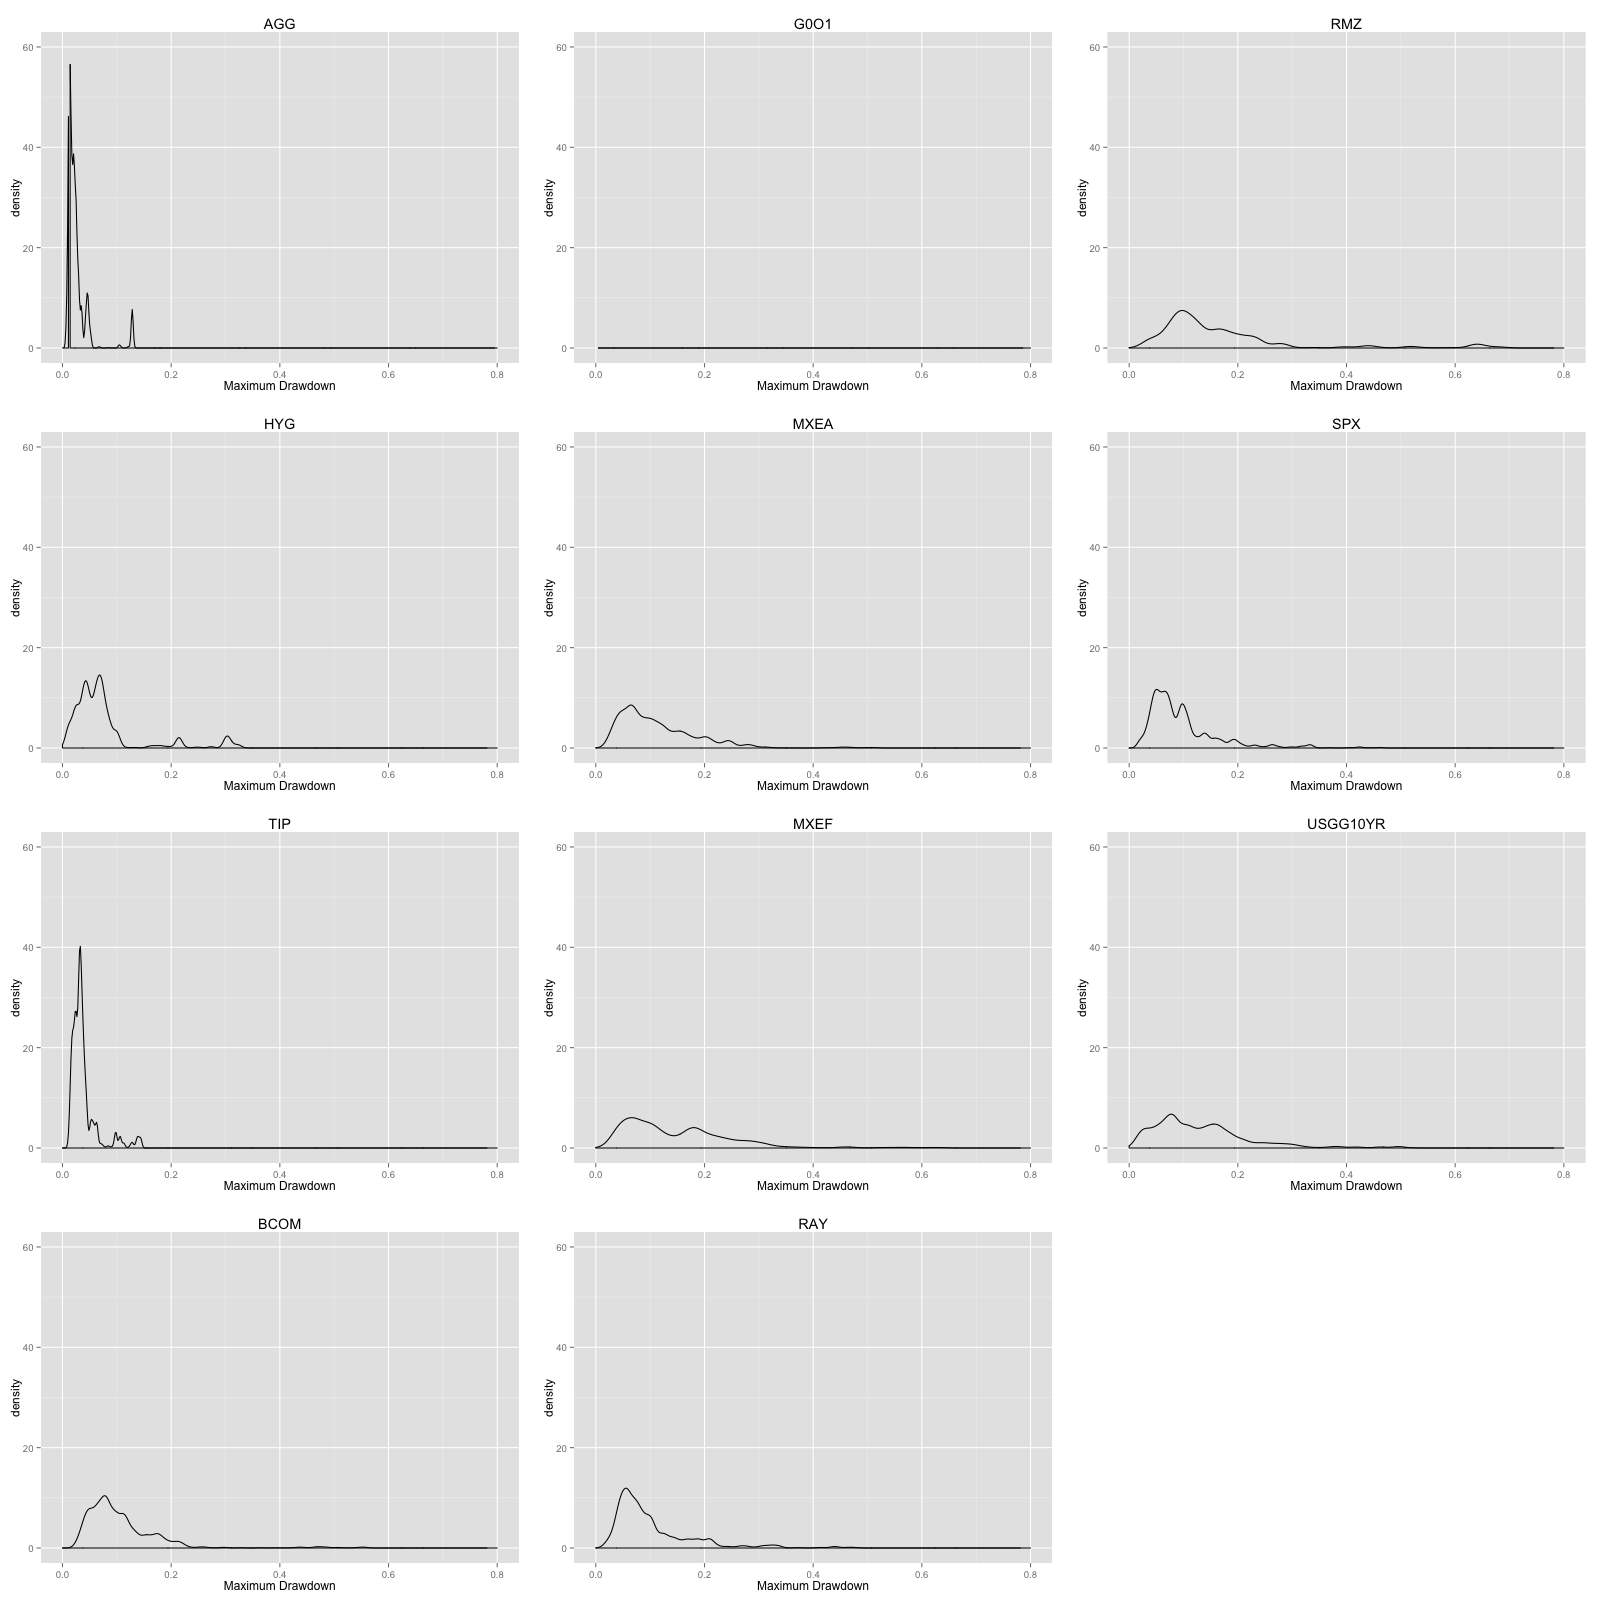
\includegraphics[width=6.5cm]{../results/maxdd_dist_mon6}
\label{fig: dist_mdd}
\end{figure}
\end{columns}
\end{frame}

%------------------------------------------------

\begin{frame}
\frametitle{Tail Mean of Maximum Drawown Distribution}
\Fontviii
\begin{table}[!h]
\centering 
\caption{tail mean of maximum drawdown distribution under 3-month and 6-month rolling window} % title of Table
\begin{tabular}{ | r || r r r || r r r |} 
 \hline
 & & 3 month & & & 6 month & \\
Asset& 0.9 & 0.95 & 0.99 & 0.9 & 0.95 & 0.99  \\
  \hline \hline
AGG &  5.60 &  7.72 & 12.84 &  8.12 & 11.45 & 12.84\\ 
HYG & 18.41 & 24.07 & 29.67 & 26.43 & 30.77 & 32.26\\ 
TIP &  7.48 &  9.90 & 13.10 & 11.14 & 12.91 & 14.39\\ 
BCOM & 18.14 & 22.54 & 38.03 & 26.61 & 33.66 & 51.74\\ 
G0O1 &  0.10 &  0.145 &  0.26 &  0.14 &  0.23 &  0.26\\ 
MXEA & 20.39 & 23.73 & 33.32 & 27.21 & 31.79 & 47.11\\ 
MXEF & 26.21 & 30.80 & 48.03 & 36.35 & 43.30 & 59.63\\ 
RAY & 20.65 & 25.64 & 35.95 & 27.81 & 34.08 & 45.08\\ 
RMZ & 37.30 & 48.41 & 63.45 & 52.04 & 62.41 & 67.61\\ 
SPX & 18.35 & 22.67 & 32.46 & 25.18 & 30.65 & 40.69\\ 
USGG10YR & 23.28 & 28.11 & 41.83 & 32.78 & 39.00 & 49.28\\
 \hline
\end{tabular}
\label{table:CED3}
\end{table}
\end{frame}

%------------------------------------------------

\begin{frame}
\frametitle{Conditional Expected Drawdown}
The conditional expected drawdown is defined as:
\begin{equation}
CED_\alpha(X_{T_n}) = \textbf{E}(\mathbf{\mu}(X_{T_n})|\mathbf{\mu}(X_{T_n}) > DT_\alpha)
\end{equation}
where $\mathbf{\mu}(X_{T_n})$ is the maximum drawdown distribution over a finite path.
We calculate the CED of various assets under 0.9, 0.95, 0.99 confidence level for different path length (3 months, 6 months, 1 year, 2 years, 5 years) separately. 
\end{frame}

%------------------------------------------------

\begin{frame}
\frametitle{Conditional Expected Drawdown}
\Fontviii
\begin{columns}[c] % The "c" option specifies centered vertical alignment while the "t" option is used for top vertical alignment

\column{.35\textwidth} % Left column and width
\textbf{Heading}
\begin{enumerate}
\item Statement
CED under 3\-month\-5\-year Rolling Window (confidence level = 0.95)
\item Example
\end{enumerate}

\column{.6\textwidth} % Right column and width
\begin{figure}[h]
\centering 
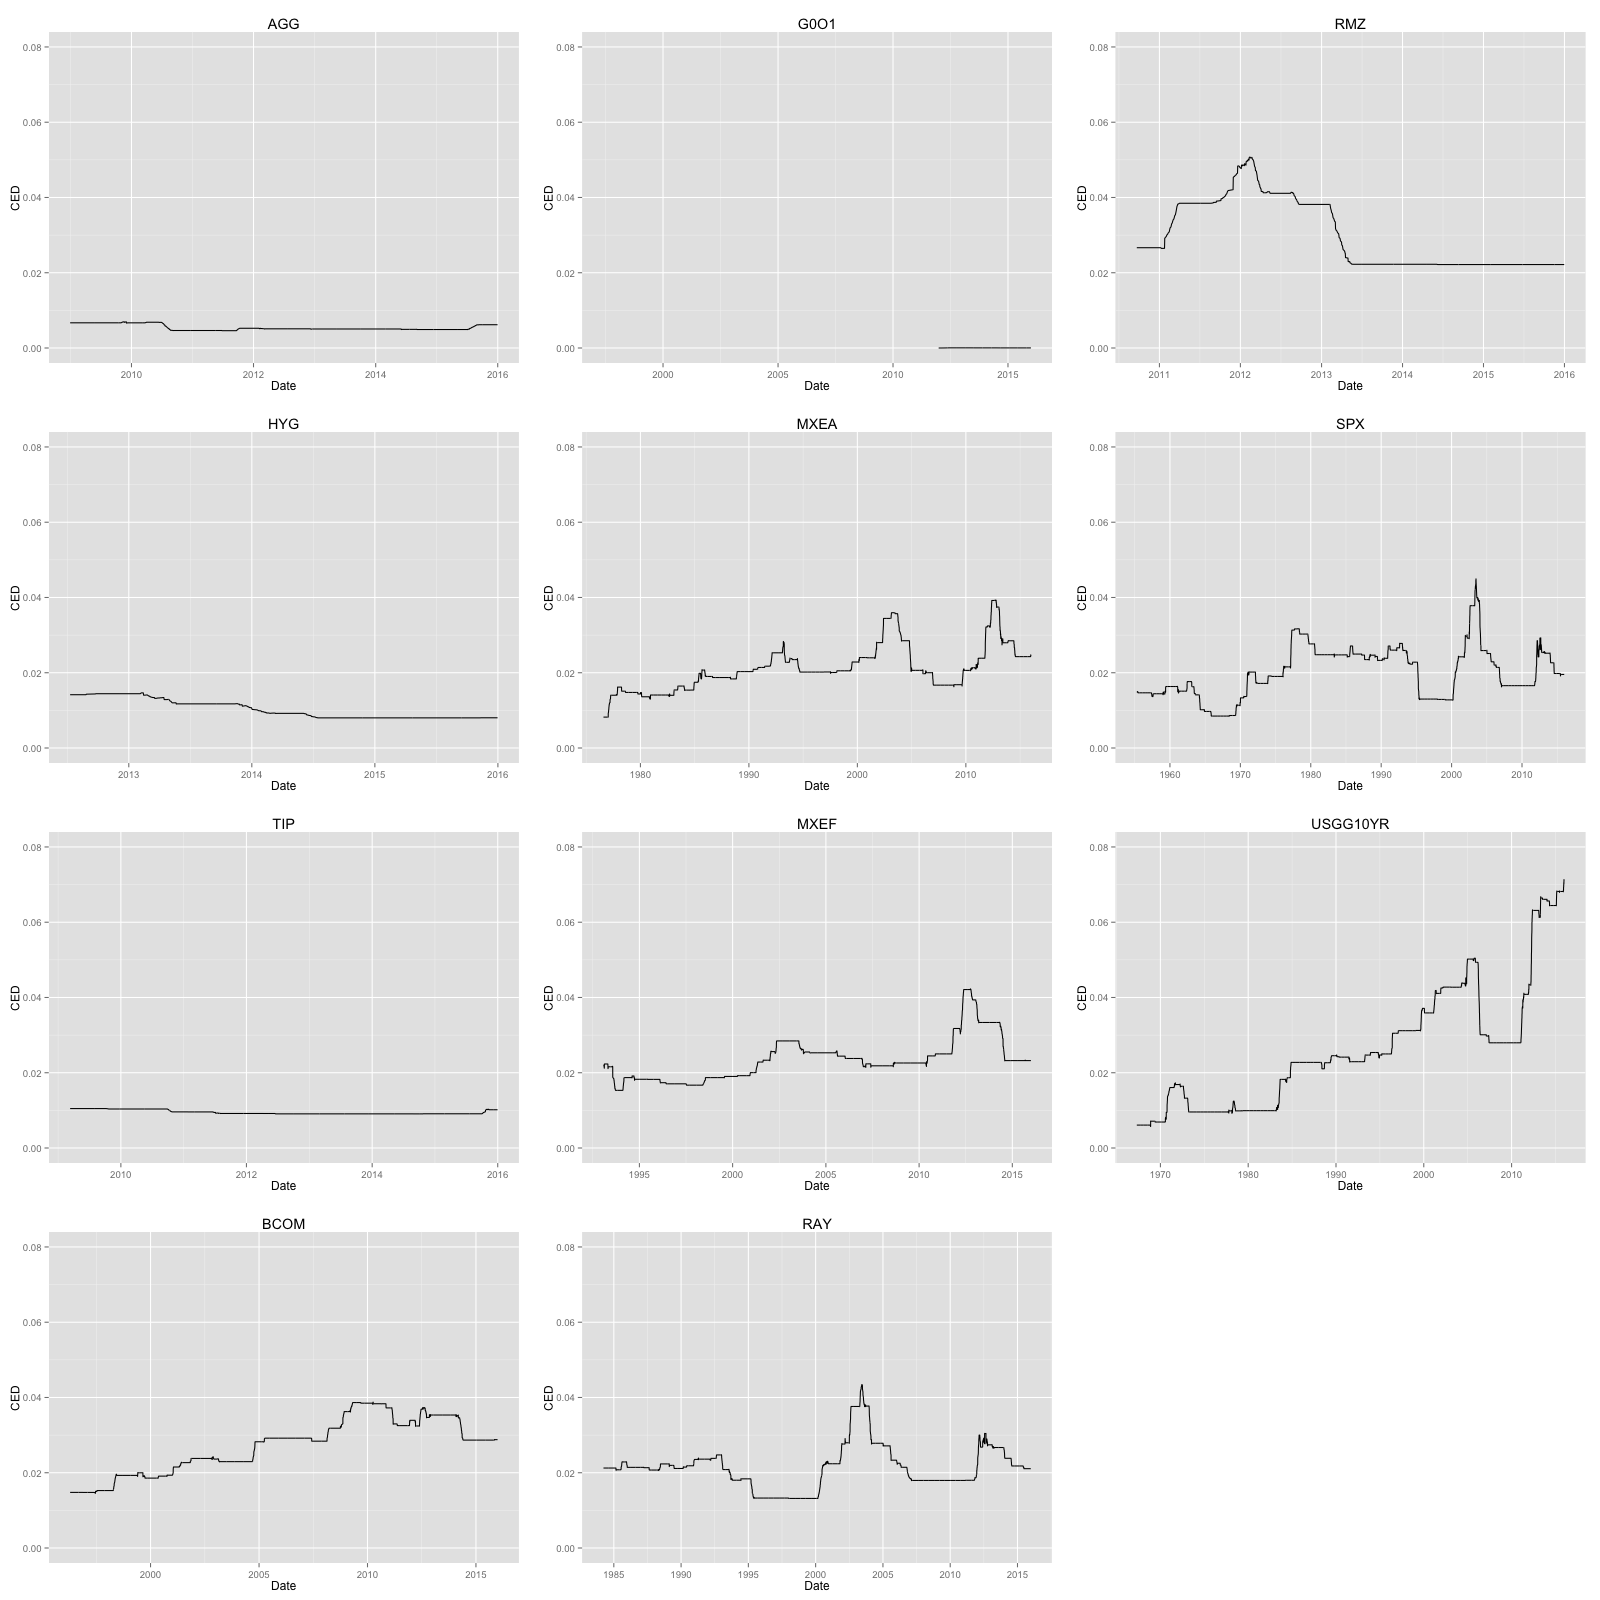
\includegraphics[width=6.5cm]{../results/CED_3mon_5yr_95}
\label{fig: CED3mon5yr95}
\end{figure}
\end{columns}
\end{frame}

%------------------------------------------------
\section{Time Varying Risk Diagnostics}
%------------------------------------------------
\subsection{Time Varying Volatility}
%------------------------------------------------

\begin{frame}
\frametitle{Time Varying Volatility}
\Fontviii
\begin{columns}[c] % The "c" option specifies centered vertical alignment while the "t" option is used for top vertical alignment

\column{.35\textwidth} % Left column and width
\textbf{Heading}
\begin{enumerate}
\item 
Volatility under 6\-month rolling window
\item Example
\end{enumerate}

\column{.6\textwidth} % Right column and width
\begin{figure}[h]
\centering 
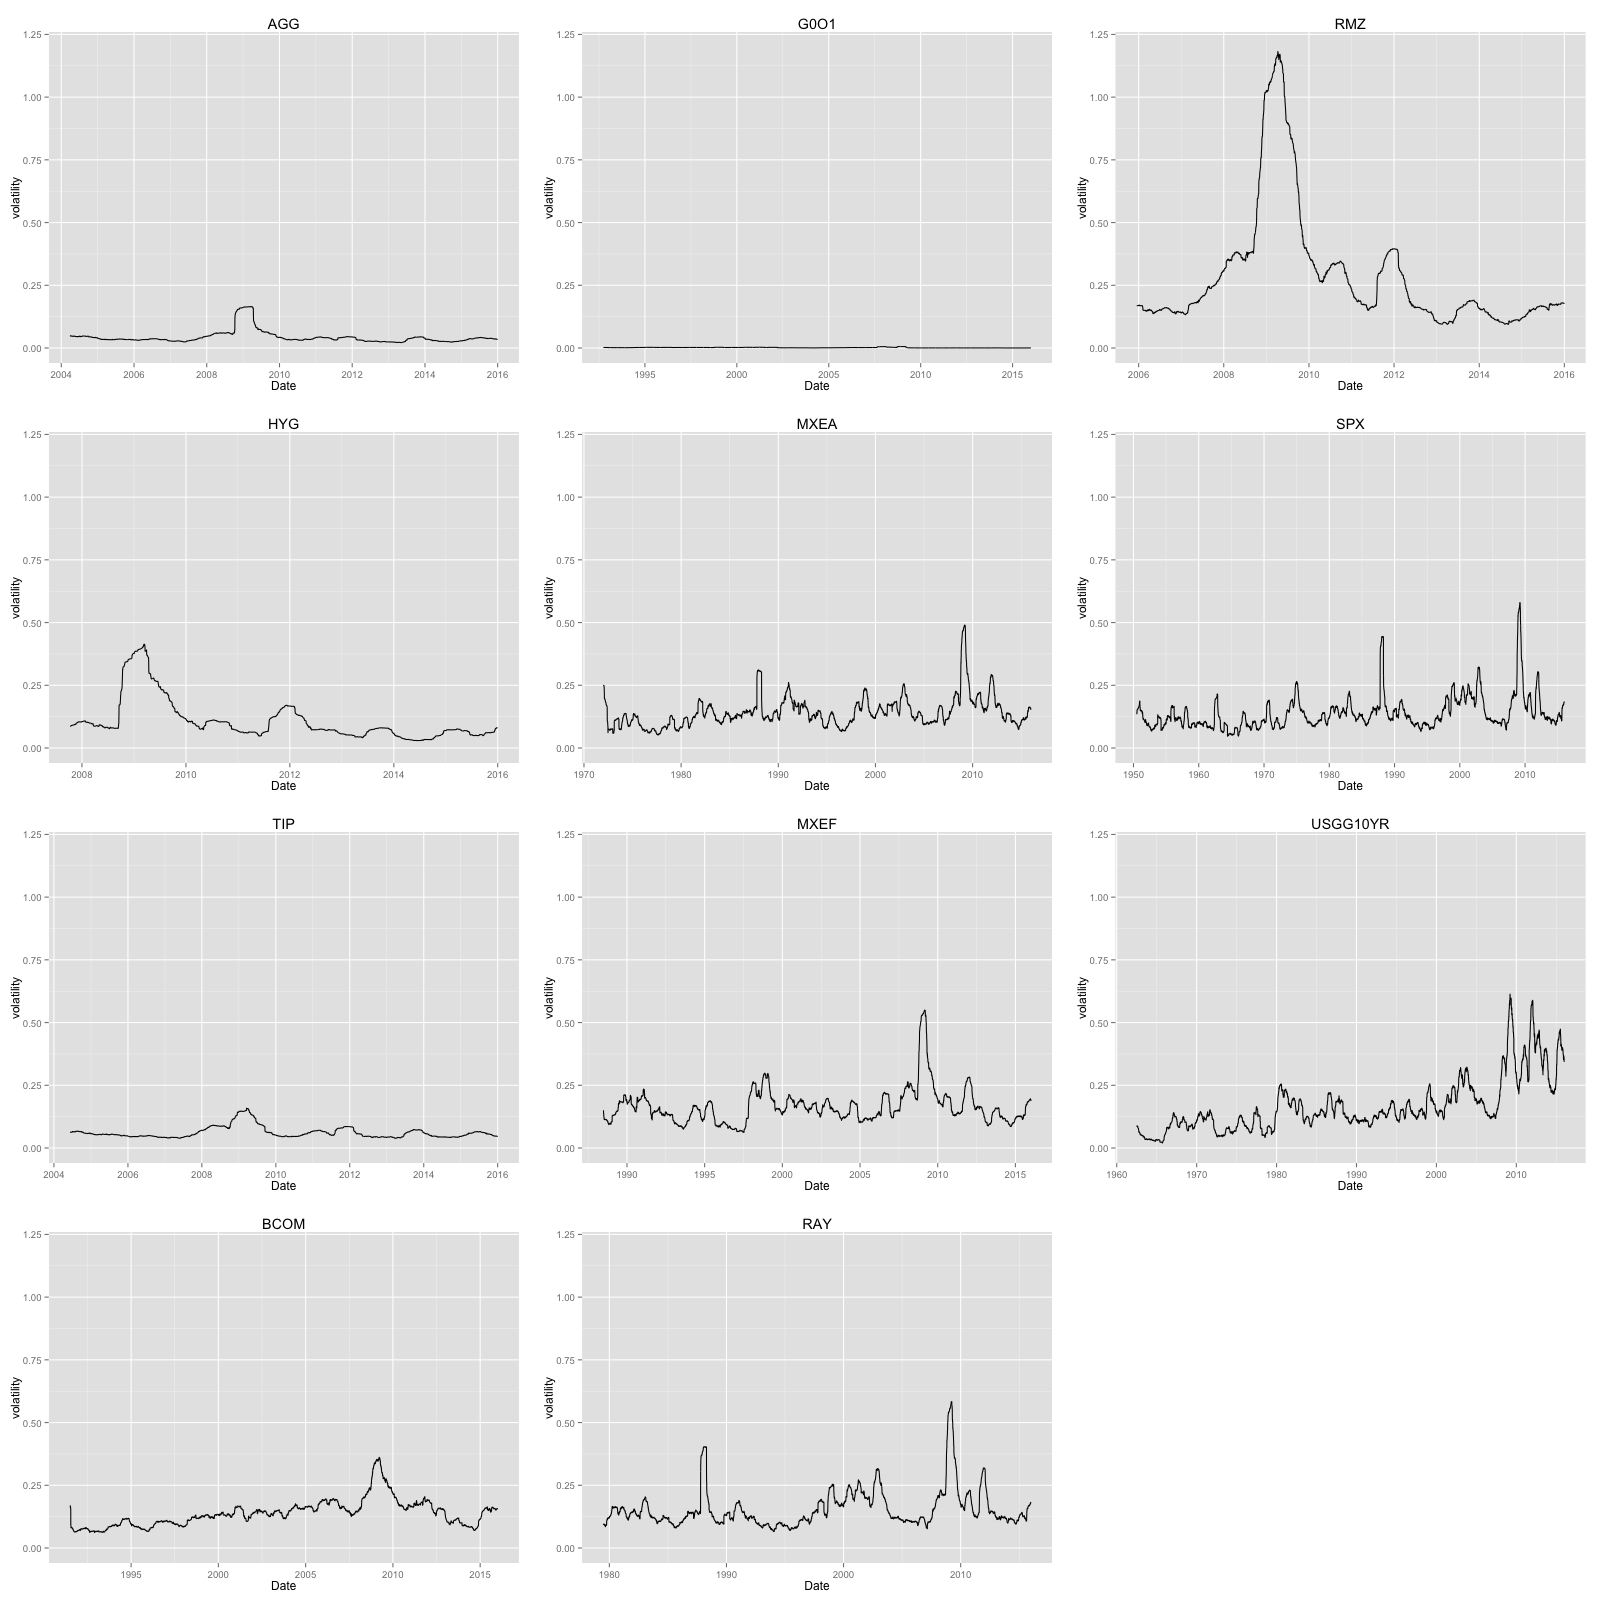
\includegraphics[width=6.5cm]{../results/volatility6mon}
\label{fig: variance6mon}
\end{figure}
\end{columns}
\end{frame}

%------------------------------------------------
\subsection{Time Varying VaR}
%------------------------------------------------

\begin{frame}
\frametitle{Time Varying VaR}
\Fontviii
\begin{columns}[c] % The "c" option specifies centered vertical alignment while the "t" option is used for top vertical alignment

\column{.35\textwidth} % Left column and width
\textbf{Heading}
\begin{enumerate}
\item VaR(\%) under 6\-month rolling window
\item Example
\end{enumerate}

\column{.6\textwidth} % Right column and width
\begin{figure}[h]
\centering 
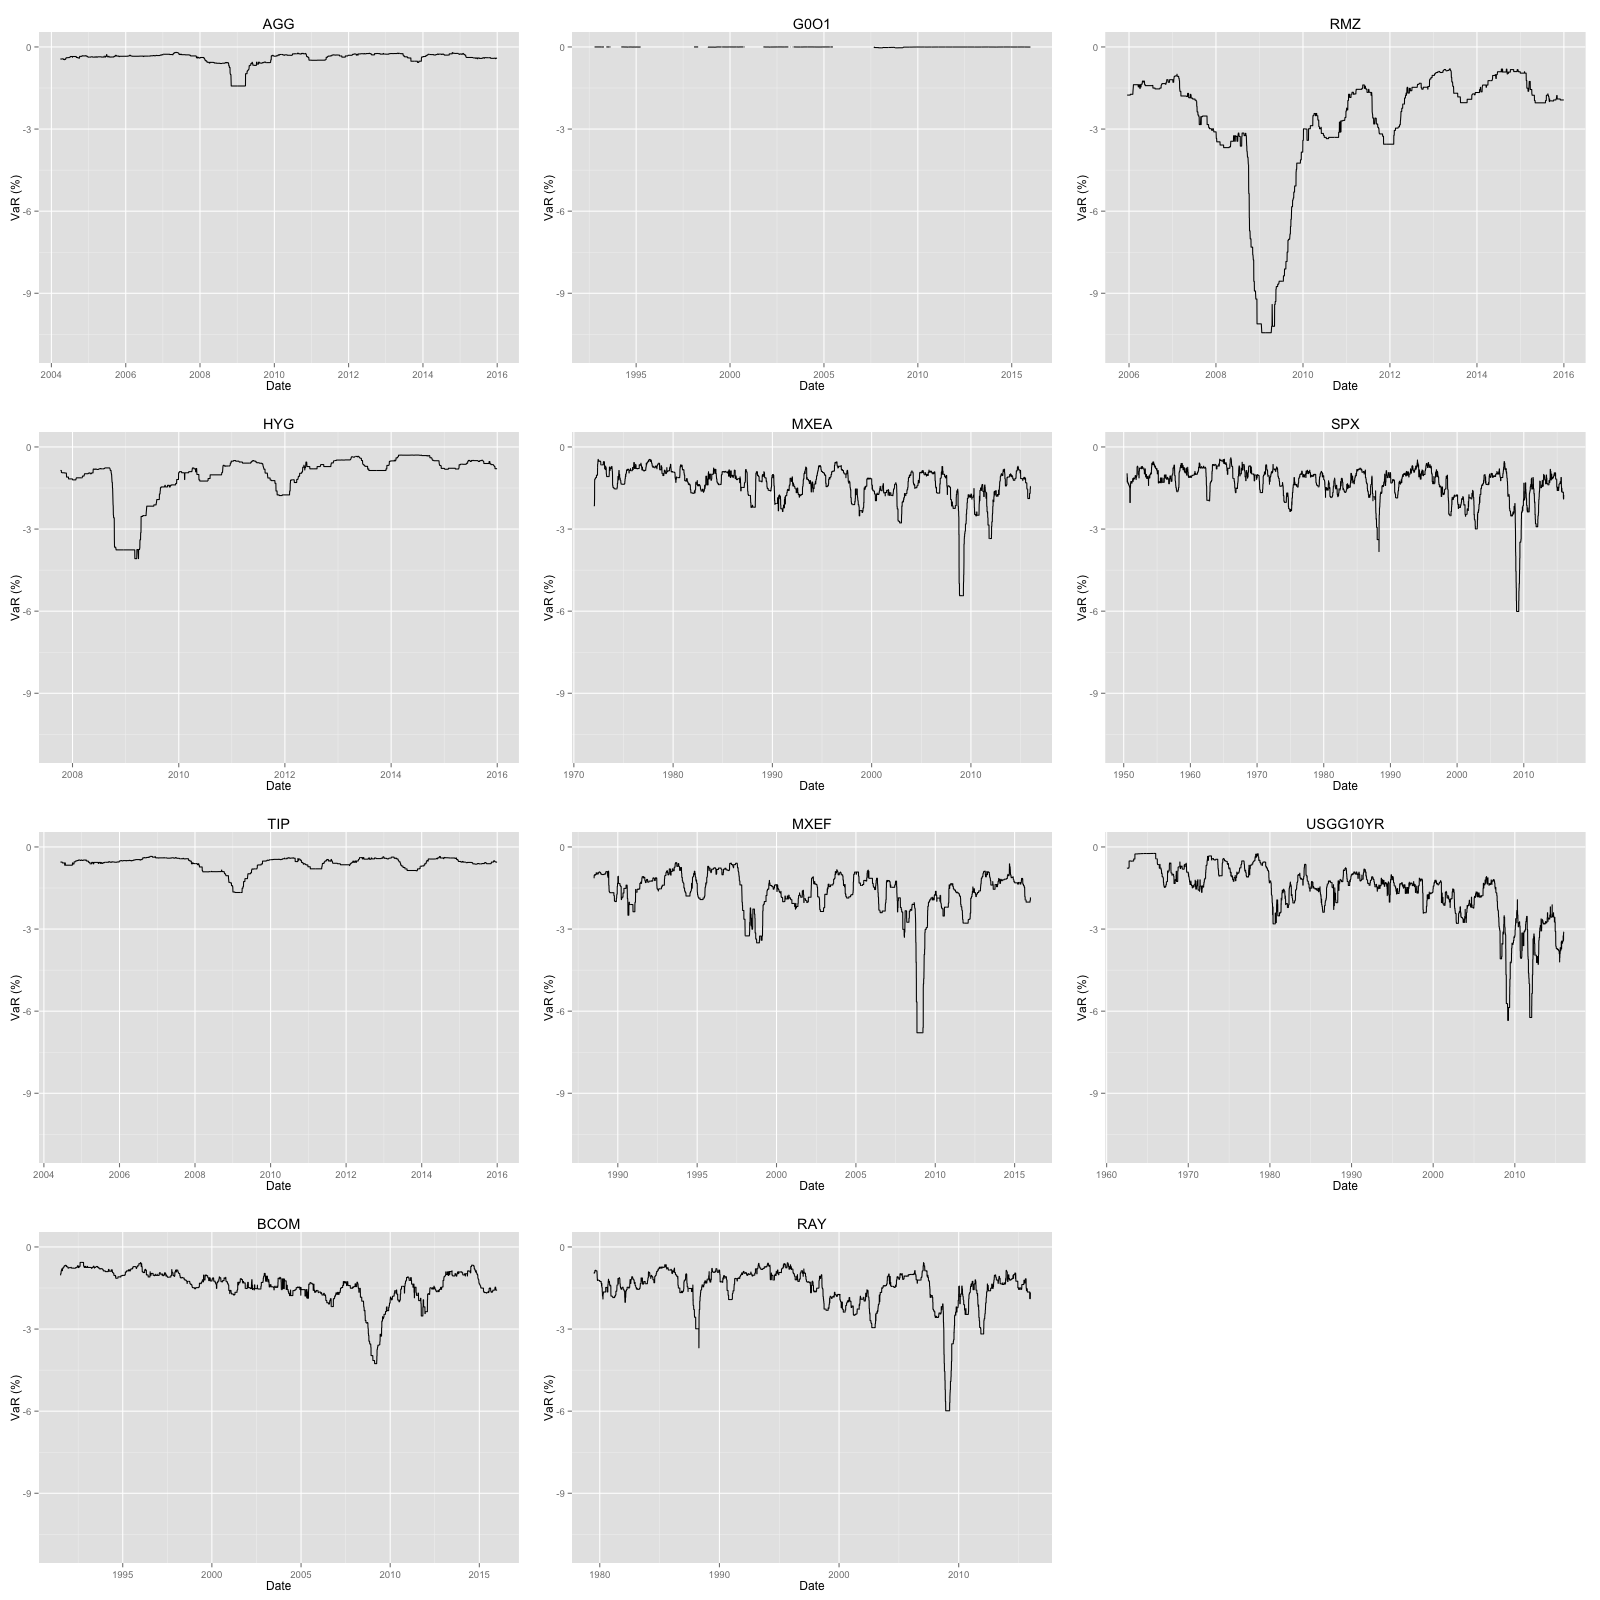
\includegraphics[width=6.5cm]{../results/VaR6mon_scaled}
\label{fig: VaR6mon}
\end{figure}
\end{columns}
\end{frame}

%------------------------------------------------
\subsection{Time Varying ES}
%------------------------------------------------

\begin{frame}
\frametitle{Time varying ES}
\Fontviii
\begin{columns}[c] % The "c" option specifies centered vertical alignment while the "t" option is used for top vertical alignment

\column{.35\textwidth} % Left column and width
\textbf{Heading}
\begin{enumerate}
\item ES(\%) under 6\-month rolling window
\item Example
\end{enumerate}

\column{.6\textwidth} % Right column and width
\begin{figure}[h]
\centering 
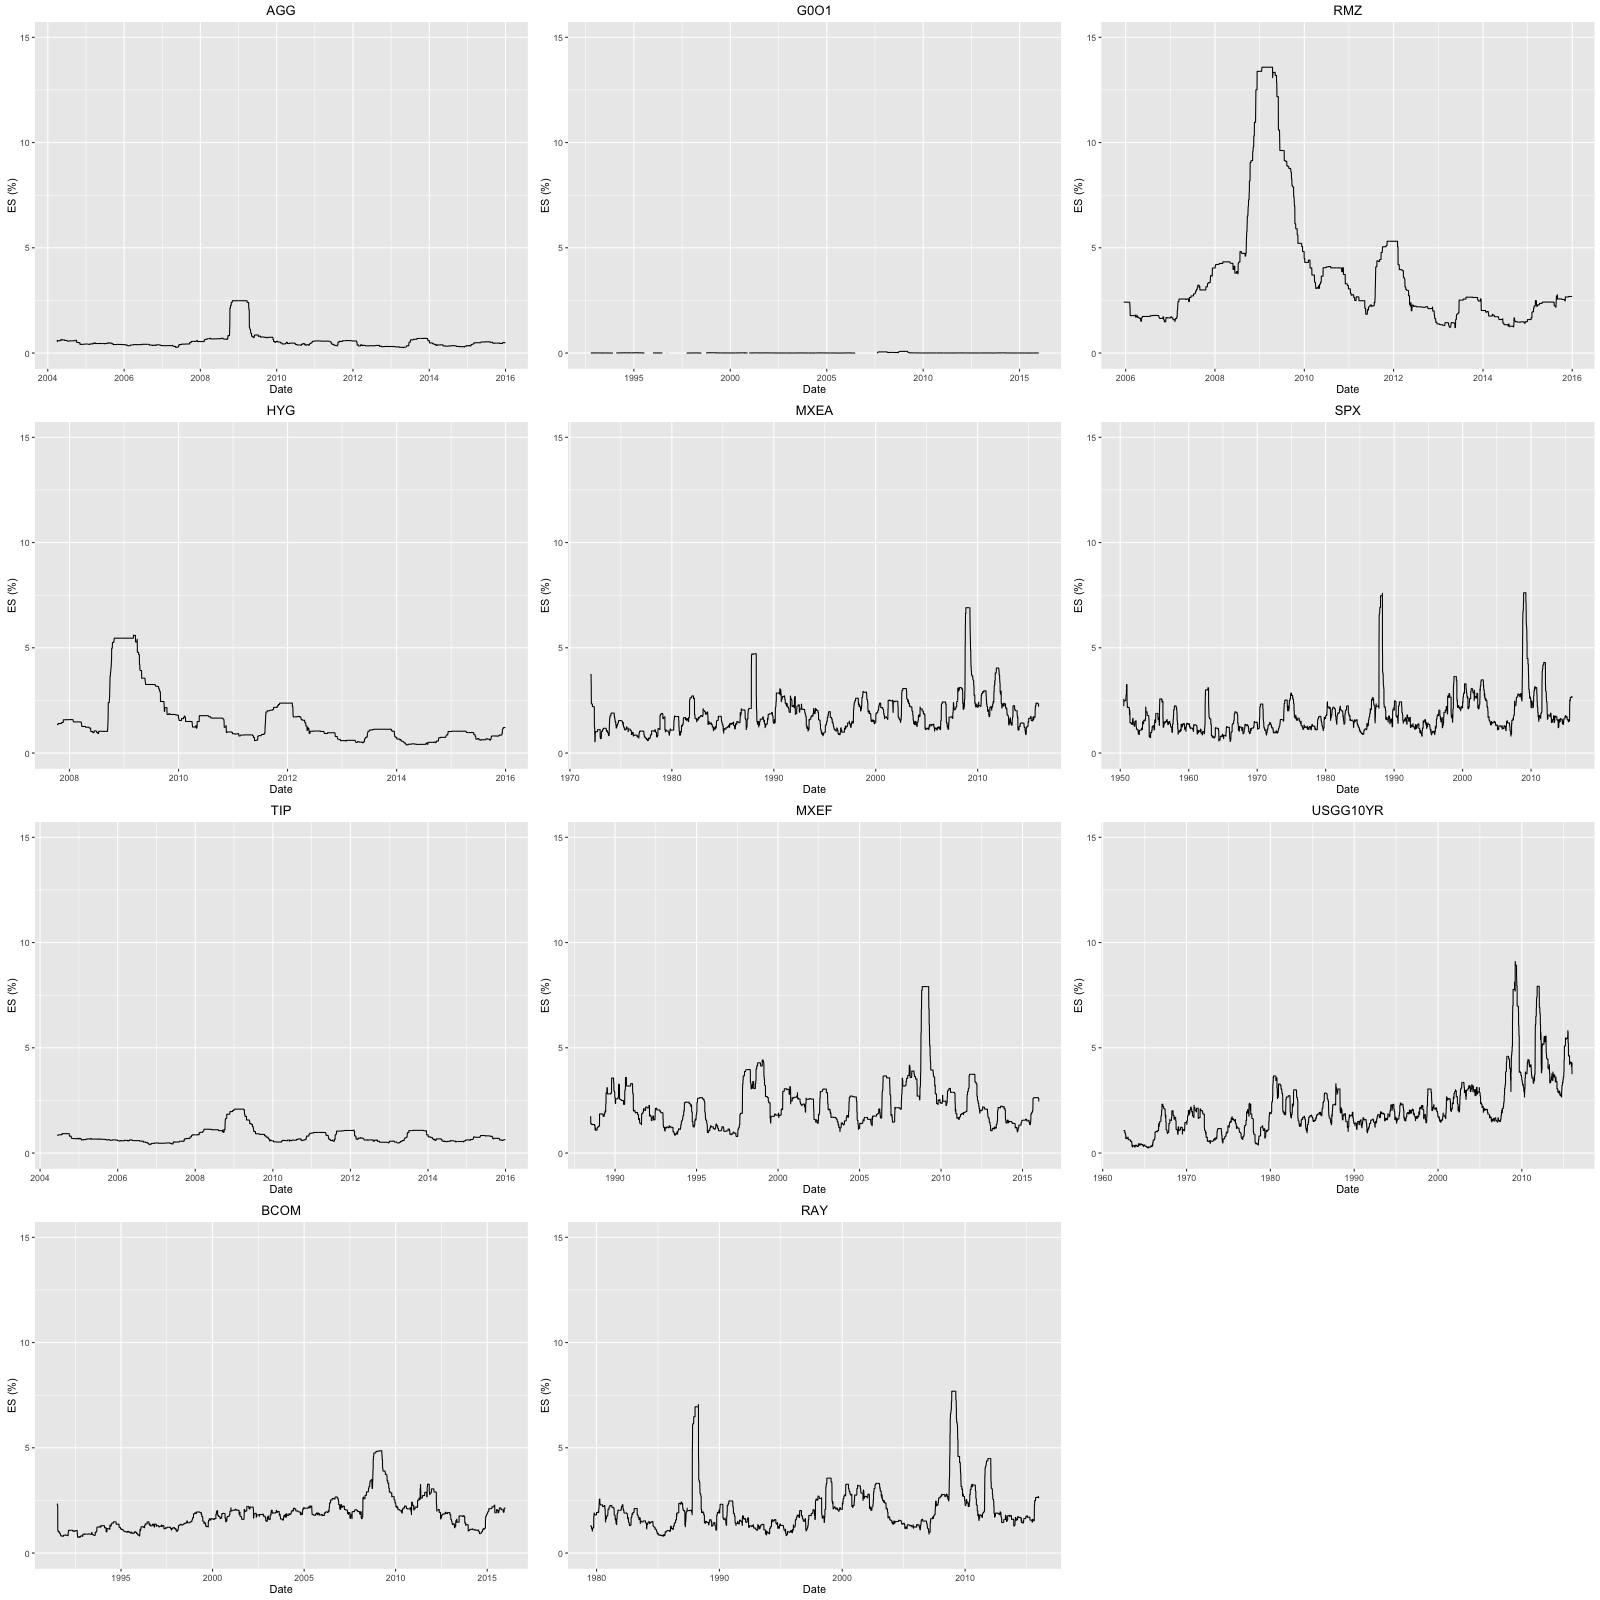
\includegraphics[width=6.5cm]{../results/ES6mon_scaled}
\label{fig: ES6mon}
\end{figure}
\end{columns}
\end{frame}

%------------------------------------------------
\section{Current Work}
%------------------------------------------------
\subsection{Time series}
%------------------------------------------------

\begin{frame}
\frametitle{}

\end{frame}

%------------------------------------------------
\subsection{Questions}
%------------------------------------------------

\begin{frame}
\Huge{\centerline{Questions}}
\end{frame}

%------------------------------------------------

\begin{frame}
\Huge{\centerline{The End}}
\end{frame}

%----------------------------------------------------------------------------------------

\end{document} 